\documentclass{article}

\title{Optimizing fusion gain through a simplified whole-device model}

\usepackage{graphicx}
\usepackage{amsmath}
\usepackage{amssymb}
\usepackage[dvipsnames]{xcolor}
\usepackage{siunitx}
\usepackage[margin=1in]{geometry}
\usepackage{parskip}
\usepackage{circuitikz}
\usepackage{bm}

\usepackage{biblatex}
\addbibresource{references.bib}

\newcommand{\jack}[1]{{\color{ForestGreen} #1}}

\begin{document}
\maketitle

\section{Introduction}

This document describes a proposed modeling problem for the summer school hackathon.
We'll first describe the physical picture and motivation, then the governing equations, and finally
the configuration of software components we'll use to investigate it.

The setting is the on-axis plasma in a Z Pinch device, bounded on one end by a cathode and on the
other by an anode.
As the Z Pinch current ramps up, and the plasma undergoes compression, on-axis current must connect
through a Langmuir sheath at both electrodes.
The dynamics of the current can be modeled as a series RLC circuit: a circuit containing a resistor,
an inductor, and a capacitor.
The RLC circuit equations let us relate the plasma current, which can be observed from the quasi-steady 
solution of our plasma kinetic equations, to the plasma voltage gap; that is, the voltage gap
across the plasma-facing electrodes.

The final piece of the picture is adiabatic compression. To a first approximation, we can assume
that the pinch is compressing adiabatically, which gives scaling relations between the plasma current
and the on-axis bulk plasma quantities, such as number density and temperature.

Putting all of these pieces together, there is a potential optimization problem to be investigated:
what combination of circuit and plasma parameters maximizes a quantity of interest such as time-integrated
neutron yield, or perhaps Q-scientific?
If the circuit model, bulk plasma model, and sheath model can all be implemented in a differentiable
program, then the optimization problem can be tackled with a derivative-based optimizer.

\begin{figure}
    \centering
    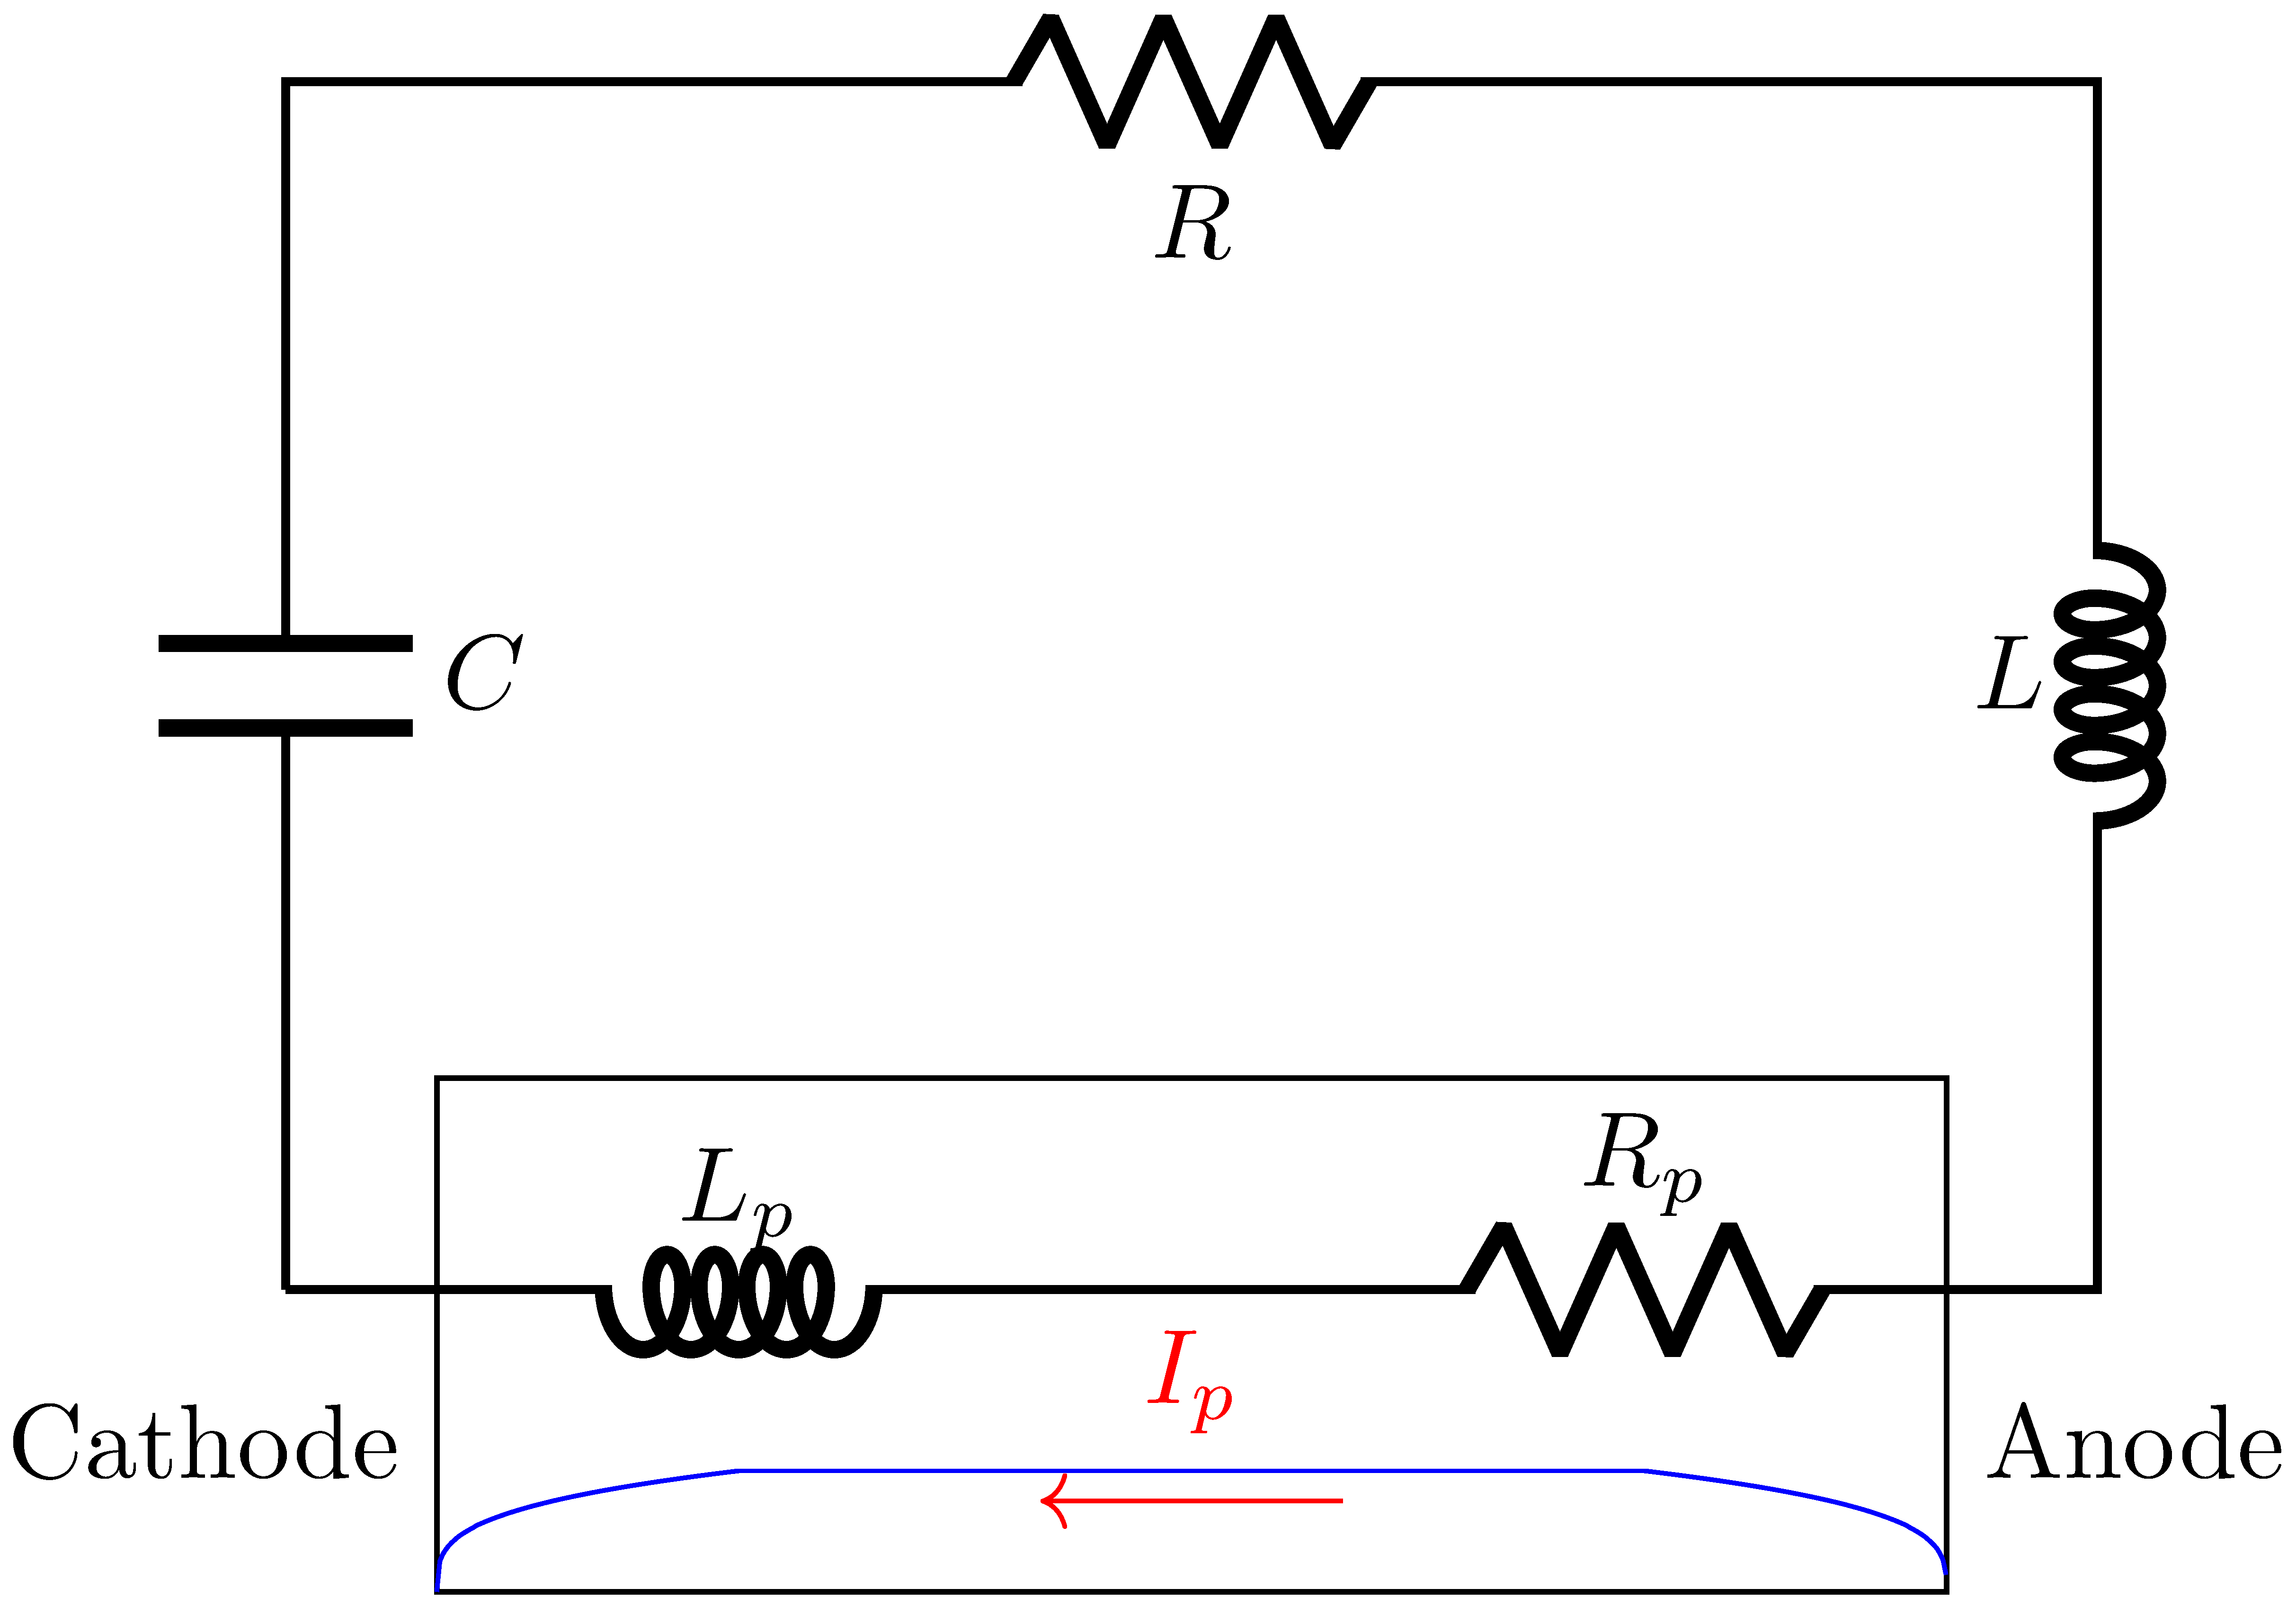
\includegraphics[width=0.6\textwidth]{images/circuit_diagram.pdf}
\end{figure}


\section{Circuit model}

This section describes the series RLC circuit equations for a discharging capacitor.
Let $Q(t)$ be the charge in the capacitor, $C$ the capacitance, $R$ the resistance,
and $L$ the total inductance of the circuit.
The total current is assumed constant throughout the circuit, and is equal to the rate of change of the charge:
\begin{align*}
    I = I_p = \dot{Q}.
\end{align*}
The voltages of each component are related by Kirchoff's voltage law
\begin{align}
V_R + V_L + V_C - V_p = 0,
\end{align}
where $V_p$ is the voltage drop across the plasma, and $V_R, V_L, V_C$ are the voltage drops across the resistor, inductor, and capacitor respectively.
The sign of $V_p$ is determined by our chosen convention, that $V_p = \phi_A - \phi_C$, where $\phi_A, \phi_C$ are the potentials at the
anode and cathode, respectively.

From the definition of capacitance we have $V_C = Q(t)/C$. From Ohm's law we have $V_R = I_p R = \dot{Q} R$, 
and $V_L = L \dot{I} = L \ddot{Q}$.
Finally, we decompose the plasma voltage into the sum of a resistive component and an inductive component:
\begin{align*}
    V_p = V_{Rp} + L_p \ddot{Q} 
\end{align*}

Combining all of the voltage terms, we obtain a second-order ODE for $Q(t)$:
\begin{align}
    \label{eqn:rlc}
    (L - L_p) \ddot{Q} + R \dot{Q} + \frac{Q}{C} = V_{Rp}
\end{align}
Equation \eqref{eqn:rlc} is not trivial to solve, because $\dot{Q}$ and $V_p$ are related
via a complex plasma model.
For now, we may consider that we have a forward plasma model that lets us compute the 
current driven by any given bias voltage:
\begin{align*}
I_p = I_p(V_p; \; T, n, L).
\end{align*}
We have included the assumed dependence on temperature, density and plasma length as parameters
for illustration purposes; in what follows we omit these parameters.

An implicit Euler scheme for \eqref{eqn:rlc} is
\begin{align}
    \label{eqn:implicit_euler}
\begin{bmatrix}
    Q^{n+1} \\ \dot{Q}^{n+1}
\end{bmatrix}
=
\begin{bmatrix}
    Q^{n} \\ \dot{Q}^{n}
\end{bmatrix}
+
\Delta t
\begin{bmatrix}
    I_p^{n+1} \\
    \frac{1}{L - L_p} \left( -Q^{n+1} / C - R I_p^{n+1} + V_{Rp}^{n+1} \right) 
\end{bmatrix}.
\end{align}
This may be solved by finding the root of the residual function
\begin{align*}
\mathcal{R} \left( \begin{bmatrix}
        Q^{n+1} \\ V_p^{n+1}
\end{bmatrix} \right) 
=
\begin{bmatrix}
    Q^{n+1} - Q^n - \Delta t I_p^{n+1} \\
    -I_p^{n+1} + \dot{Q}^n + \frac{\Delta t}{L - L_p} \left( -Q^{n+1}/C - R I_p^{n+1} - V_{Rp}^{n+1} \right) 
\end{bmatrix},
\end{align*}
where $I_p^{n+1} = I_p(V_p^{n+1})$, and the resistive component of the plasma voltage must be solved for:
\begin{align*}
    V_{Rp}^{n+1} &= V_p^{n+1} - L_p \ddot{Q} \\
                 &= V_p^{n+1} - \frac{L_p}{L - L_p} \left( -\frac{Q^{n+1}}{C} - R I_p^{n+1} - V_{Rp}^{n+1} \right),
\end{align*}
giving
\begin{align*}
    V_{Rp}^{n+1} = \left( 1 - \frac{L_p}{L - L_p} \right)^{-1} \left( V_p^{n+1} - \frac{L_p}{L - L_p} \left( -\frac{Q^{n+1}}{C} - R I_p^{n+1} \right) \right).
\end{align*}

The root of the residual $\mathcal{R}$ can be found by a Newton iteration.
In a differentiable programming environment, such a routine is trivial to write,
but it relies on the ability to evaluate the gradient of $I_p$.
This indicates that for our circuit solve, we require an end-to-end differentiable 
kinetic plasma simulation.


\section{Incorporating plasma compression, resistive heating, and radiative cooling}

As the capacitor discharge modeled by the above RLC circuit equations proceeds, the plasma
between the electrode gap is far from static.
Its bulk properties (principally density and temperature) change, which drive increasing
fusion yield.
For the purposes of this modeling exercise, we include three effects:
\begin{itemize}
    \item Adiabatic compression of the plasma on-axis
    \item Resistive heating of the plasma by the plasma current
    \item Radiative cooling of the plasma, principally by so-called Bremsstrahlung radiation
\end{itemize}
We incorporate these effects into an extended ODE model for current, temperature, and density,
with the following time-splitting structure:
\begin{align*}
\frac{d}{dt} \begin{pmatrix}
Q \\ I_p \\ T \\ n
\end{pmatrix}
=
\begin{pmatrix}
I \\ \ddot{Q} \\ 0 \\ 0
\end{pmatrix}
+
\begin{pmatrix}
0 \\ 0 \\
\left( \frac{d T}{dt} \right)_{rad} + \left( \frac{d T}{dt} \right)_{\eta} \\
0
\end{pmatrix}
+
\begin{pmatrix}
0 \\ 0 \\
\left( \frac{dT}{dt} \right)_{comp} \\
\left( \frac{dn}{dt} \right)_{comp}
\end{pmatrix}.
\end{align*}
The idea is to step each term separately. 
We begin with an Implicit Euler step of the current terms, described above,
followed by an explicit solve of the radiative and resistive terms.
Finally, we assume that the compression step occurs adiabatically and reaches
radial force balance much faster than a single timestep.

\subsection{Resistive heating}
Resistive heating of a plasma follows a volumetric analogue to Ohm's law.
Heating per unit volume is given by
\begin{align*}
    P_{\eta} = \eta j^2,
\end{align*}
where $\eta$ can be estimated by the (corrected) Spitzer resistivity \cite{goldstonIntroductionPlasmaPhysics1995a}
\begin{align*}
    \eta = \frac{1}{1.96} \frac{\sqrt{2} m_e^{1/2} Z e^2 \ln \Lambda}{12 \pi^{3/2} \epsilon_0^2 T^{3/2}},
\end{align*}
and we will use the average current density,
\begin{align*}
j = \frac{I}{\pi a^2},
\end{align*}
where $a = \sqrt{N / \pi n}$ is the pinch radius.

Dividing by the volumetric density, we get
\begin{align*}
    \left( \frac{dT}{dt} \right)_\eta = \frac{P_{\eta}}{n} = \frac{\eta j^2}{n}.
\end{align*}

\subsection{Radiative losses}
The primary radiative cooling of interest in a fusion plasma is bremsstrahlung radiation.
This form of radiation is produced by electrons accelerating (or decelerating), and in a
plasma is associated with Coulomb collisions between ions and electrons.

The approximate volumetric power density of bremsstrahlung losses in a plasma is \cite{goldstonIntroductionPlasmaPhysics1995a}
\begin{align*}
    P_{br}[\unit{eV s^{-1} m^{-3}}] = 1.06 \times 10^{-19} Z^2 n_{e[\unit{m^{-3}}]} n_{i[\unit{m^{-3}}]} T_{[\unit{eV}]}^{1/2}.
\end{align*}
We can assume $n_e = Z n_i$, and for a hydrogen or D-T plasma we have $Z = 1$.
Once again dividing by the volumetric density, we get
\begin{align*}
    \left( \frac{dT}{dt} \right)_{rad} = -\frac{P_{br}}{n}
\end{align*}

\subsection{Adiabatic compression}

The principal effect of increasing the plasma current is to compress the plasma: as it seeks
to maintain force balance between the confining magnetic field and its own thermal pressure,
the latter increases.
By making the reasonable assumption that this process is \emph{adiabatic}, meaning that
it occurs slowly enough that no shock waves appear, we can derive scaling relations between
two states that are connected by a compression event.
Denoting the two states by subscripts 1 and 2, \cite{shumlakShearedFlowStabilizedZPinch2012}
provides the following adiabatic scaling relations.
We assume that the linear density $N$ is constant.

For any plasma in radial force balance, the temperature is related to current by
\begin{align*}
\frac{T_2}{T_1} = \frac{I_2^2}{I_1^2}.
\end{align*}
The volumetric density scales as
\begin{align*}
    \frac{n_2}{n_1} = \left( \frac{T_2}{T_1} \right)^{\frac{1}{\gamma-1}},
\end{align*}
where $\gamma$ is the adiabatic constant, which we will take to be $5/3$.

\subsection{Putting it all together}

To advance from time $t^n$ to time $t^{n+1}$ we use the following scheme:
\begin{align*}
    &\begin{pmatrix}
        Q^{n+1} \\
        I_p^{n+1}
    \end{pmatrix} = IE \begin{pmatrix}
    Q^n \\ I_p^n
    \end{pmatrix}, \\
    &T' = T^n + \Delta t \left( \frac{P_{\eta}^n}{n^n} - \frac{P_{br}^n}{n^n} \right) \\
    &T^{n+1} = (I_p^{n+1}/I_p^n)^2 T^n \\
    &n^{n+1} = (T^{n+1} / T')^{\frac{1}{\gamma-1}} n^n
\end{align*}
where $IE$ represents a single timestep of the Implicit Euler scheme \eqref{eqn:implicit_euler}.
To tell a story about the final three equations, $T'$ represents the temperature after
a single timestep of non-adiabatic heating and cooling.
Depending on whether resistive heating or radiative cooling dominates, the plasma is either over- or under-pressured
at this point.
It then undergoes expansion or compression until it is in radial force balance again.
Its temperature in radial equilibrium is independent of $T'$, and depends only on the ratio of currents
between times $t^{n+1}$ and $t^n$.
However, the adiabatic expansion or compression is between states with temperatures $T'$ and $T^{n+1}$,
so that the ratio of volumetric densities is determined by $T'$.

\section{Vlasov discretizations}

The governing kinetic equation for our study is the 1D1V Vlasov-Dougherty-Fokker-Planck equation in
the ``flexible plasma normalization'' \cite{millerMultispecies13momentModel2016}:
\begin{align}
    \label{eqn:vlasov_fp}
    \partial_t f_s + v \partial_x f_s + (\omega_c \tau) \frac{Z_s}{A_s} E \partial_v f_s &= Q(f_s) \\
                                                                                         &= \sum_{s'} Q_{s s'}(f_s)  \\
                                                                                         &= (\nu_p \tau) \sum_s \nu_{s s'} \partial_v \left( \frac{T_{s s'}}{m_s} \partial_v f_s + (v - u_{s s'}) f_s \right).
\end{align}
The normalization constants appearing in this equation are as follows:
\begin{itemize}
    \item $Z_s$ and $A_s$ are the normalized charge and mass of species $s$, expressed in units of the proton charge and mass.
    \item $\omega_c \tau$ is the normalized reference proton cyclotron frequency in a field $B_0$ which would give unit plasma beta: $|B_0|^2 / 2 \mu_0 = n_0 T_0$.
    \item $\nu_p \tau$ is the normalized proton collision frequency.
\end{itemize}
For now we can take these normalization constants as given; we will need to concern ourselves with their definitions when we
move on to translating a specific physical problem into our equation setup.

Equation \eqref{eqn:vlasov_fp} is coupled to the normalized Gauss's law,
\begin{align}
\partial_x E = \frac{(\omega_p \tau)^2}{\omega_c \tau} \rho_c,
\end{align}
where
\begin{align}
    \rho_c = \sum_s Z_s \int f_s \,\mathrm{d} v
\end{align}
is the charge density.
We will use the elliptic form of Gauss's law,
\begin{align}
\partial_x^2 \phi = -\frac{(\omega_p \tau)^2}{\omega_c \tau} \rho_c,
\end{align}
with $E = -\partial_x \phi$.

\subsection{Domain and boundary conditions}

We'll use a physical domain of length $L_x$, which by convention extends from $-L_x/2$ to $L_x/2$.

\subsubsection{Absorbing wall}
The simplest boundary condition that will produce a Langmuir sheath is the absorbing wall
boundary condition. At a spatial boundary $x_b$ with outward normal vector $\mathbf{n}(x_b)$, we have
\begin{align}
    f_s^b(x_b, v) = \mathbf{1}_{\mathbf{n}(x_b) \cdot v < 0} f_s(x_, v),
\end{align}
where $\mathbf{1}$ is the indicator function.

\subsection{Robust conservative DLR scheme}

This is a multispecies extension of the single-species scheme with Legendre weight function 
described in \cite{coughlinRobustConservativeDynamical2024}.
We begin by expanding each species distribution function as a sum of a macro and micro component:
\begin{align*}
f_s(x, v, t) = \mathcal{N}_s(x, v, t) + g_s(x, v, t).
\end{align*}
For each species, let $v_{ts} = \sqrt{T_0 / A_s}$ be the reference thermal velocity.
The velocity domain is chosen as some fixed number of thermal velocities:
\begin{align*}
    \Omega_{vs} = [-v_{max,s}, v_{max,s}],
\end{align*}
with the constant weight function $w(v) = \frac{1}{v_{max,s}}$.
The orthonormal polynomial family is the scaled Legendre polynomials,
\begin{align*}
    p_{0s}(v) &= \sqrt{\frac{1}{2}} \\
    p_{1s}(v) &= \sqrt{\frac{3}{2}} \frac{v}{v_{max,s}} \\
    p_{2s}(v) &= \sqrt{\frac{5}{8}} \left( 3 \left( \frac{v}{v_{max,s}} \right)^2 - 1 \right)  \\
    p_{3s}(v) &= \sqrt{\frac{7}{8}} \left( 5 \left( \frac{v}{v_{max,s}} \right)^3 - 3 \frac{v}{v_{max,s}} \right). 
\end{align*}

In a multispecies context, we must derive expressions for the momentum and energy transfer between
species due to collisions.
This will require a modification to equation (2.12) of \cite{coughlinRobustConservativeDynamical2024}.

For the zeroth moment, we have
\begin{align*}
    \int_{\Omega_v} p_{0s}(v) Q_{s s'}(f_s) \, \mathrm{d} v &= 0
\end{align*}
by conservation of particles.
For the first moment,
\begin{align*}
    \int_{\Omega_v} p_{1s}(v) Q_{s s'} (f_s) \, \mathrm{d} v &= (\nu_p \tau) \nu_{s s'} \int_{\Omega_v} p_{1s}(v)  \partial_v \left( \frac{T_{s s'}}{A_s} \partial_v f_s + (v - u_{s s'}) f_s \right)  \, \mathrm{d} v \\
                                                             &= -(\nu_p \tau) \nu_{s s'} \int_{\Omega_v} p'_{1s}(v) \left( \frac{T_{s s'}}{A_s} \partial_v f_s + (v - u_{s s'}) f_s \right) \, \mathrm{d} v \\
                                                             &= -(\nu_p \tau) \nu_{s s'} d_{10} \int_{\Omega_v} p_{0s}(v) \left( \frac{T_{s s'}}{A_s} \partial_v f_s + (v - u_{s s'}) f_s \right) \, \mathrm{d} v \\
                                                             &= -(\nu_p \tau) \nu_{s s'} d_{10} \int_{\Omega_v} [ v p_{0s}(v) - u_{s s'} p_{0s}(v) ] f_s \, \mathrm{d} v \\
                                                             &= -(\nu_p \tau) \nu_{s s'} d_{10} \int_{\Omega_v} [ a_0 p_{1s} (v) + b_0 p_{0s}(v) - u_{s s'} p_{0s}(v) ] f_s \, \mathrm{d} v \\
                                                             &= -(\nu_p \tau) \nu_{s s'} d_{10} \left[ a_0 f_{1s} + b_0 f_{0s} - u_{s s'} f_{0s} \right].
\end{align*}
For the second moment,
\begin{align*}
    \int_{\Omega_v} p_{2s}(v) Q_{s s'} (f_s) \, \mathrm{d} v &= (\nu_p \tau) \nu_{s s'} \int_{\Omega_v} p_{2s}(v)  \partial_v \left( \frac{T_{s s'}}{A_s} \partial_v f_s + (v - u_{s s'}) f_s \right)  \, \mathrm{d} v \\
&= -(\nu_p \tau) \nu_{s s'} \int_{\Omega_v} p_{2s}'(v) \left( \frac{T_{s s'}}{A_s} \partial_v f_s + (v - u_{s s'}) f_s \right)  \, \mathrm{d} v \\
&= -(\nu_p \tau) \nu_{s s'} \int_{\Omega_v} [d_{21} p_{1s}(v) + d_{20} p_{0s}(v)] \left( \frac{T_{s s'}}{A_s} \partial_v f_s + (v - u_{s s'}) f_s \right) \, \mathrm{d} v \\
&= -(\nu_p \tau) \nu_{s s'} \int_{\Omega_v} \left[ -d_{21} \frac{T_{s s'}}{A_s} p'_{1s}(v) + d_{21} p_{1s}(v) (v - u_{s s'}) + d_{20} p_{0s}(v) (v - u_{s s'}) \right] f_s  \, \mathrm{d} v \\
&= -(\nu_p \tau) \nu_{s s'} \left[ -d_{21} d_{10} \frac{T_{s s'}}{A_s} f_{0s} + d_{21} \left( a_1 f_{2s} + b_1 f_{1s} + a_0 f_{0s} - u_{s s'} f_{1s} \right) + d_{20} \left( a_0 f_{1s} + b_0 f_{0s} - u_{s s'} f_{0s} \right)   \right] 
\end{align*}

The macro equations are therefore
\begin{align*}
\partial_t \begin{pmatrix}
f_0 \\ f_1 \\ f_2
\end{pmatrix}_s
\end{align*}

\end{document}
